% ------------------------------- Section ---------------------------------- %
%%                                                                          %%
%%%                                                                        %%%
%%                                                                          %%
% -------------------------------------------------------------------------- %
\section{Testing on expanding polyurethane foam application}
\label{sec:0Dmodel}

In this section, the work on integrating the sub-models, recipes and adaptors
originating from WP1-3 is presented. The target application is an expanding
polyurethane foam.  A novel modelling approach, based on the solution of the
population balance equation ({\PopulationBalanceEquation}), is used and applied
for the first time to the simulation of expanding polyurethane foams.  The model
will be validated against experiments from the literature in WP 6.

Polyurethane foams are widely used materials, employed in many different
applications, and almost always manufactured into useful objects via direct
injection expanded foam molding
\cite{woods_1990,oertel_and_abele_1994,klempner_and_frisch_1991}.  The final
characteristics (i.e. thermal and mechanical properties) of the manufactured
objects highly depend on the final bubble (or cell) size distribution
({\BubbleSizeDistribution}) of the foam \cite{gibson_and_ashby_1999}.  This is
determined by the initial chemical recipe (i.e. isocyanate, polyol and blowing
agents structure and concentration, catalyst and surfactant type and
concentration), the injection dynamics and the flow history of the foam into the
mold.  However, the relationship between the process conditions and the final
foam characteristics is highly empirical and the development of mathematical
models is identified as the most efficient way to establish a more reliable and
quantitative approach to the problem
\cite{niyogi_and_kumar_etal_2014,beverte_2014,shen_and_zaho_etal_2014,zhao_and_gordon_etal_2013,mosanenzadeh_and_naguib_etal_2013,zhou_and_huang_etal_2006,tesser_and_deserio_etal_2004,lo_and_reible_etal_1994}.
Our objective is to develop a three-dimensional model, based on computational
fluid dynamics (CFD), capable of simulating the mold filling process.  The model
also incorporates a population balance equation ({\PopulationBalanceEquation})
that describes the evolution of the {\BubbleSizeDistribution} due to bubble
growth, caused in turn by physical and chemical blowing agents, and bubble
coalescence, caused by shear-induced bubble collisions.  The combined use of
{\PopulationBalanceEquation} and CFD was demonstrated to be a very useful tool
for the simulation of many different multi-phase systems
\cite{marchisio_and_fox_2013} and seems a very promising approach also for
polyurethane foams.  Before developing the full {\PopulationBalanceEquation}-CFD
model and applying it to the three-dimensional simulation of real
industrial-scale foaming processes, the {\PopulationBalanceEquation} model is
firstly formulated, implemented in a simpler zero-dimensional framework and
partially validated with experiments taken from the literature
\cite{baser_and_khakhar_1994_a,baser_and_khakhar_1994_b,greier_and_piesche_etal_2009}.
The model accounts for the progress of the polymerisation process, between
polyol and isocyanate, by tracking the evolution of the gelling reaction.  The
presence of a physical blowing agent is also accounted for, together with the
presence of a chemical blowing agent (i.e. water), and their effect on the
{\BubbleSizeDistribution} is accounted for by solving the
{\PopulationBalanceEquation} with the efficient quadrature method of moments
({\QuadratureMethodOfMoments}) \cite{marchisio_and_fox_2013}.  The remainder of
the paper is as follows: after a short description of the model equations, the
operating conditions and investigated test cases are discussed.  Then, results
are presented and some significant conclusions are drawn.
% ..............................- Subsection -.............................. %
%%                                                                          %%
% .......................................................................... %
\subsection{Governing equations}
%
For clarity, this section starts with a list of the main simplification assumptions employed in the formulation of the baseline model. 
It must be noted that since this work tackles a mathematically and physically complex problem with limited information from the literature, some of the following simplifications are required. 
This baseline model treats the foam as perfectly mixed with a zero-dimensional "lumped" model. 
The model assumes that the foaming process starts after mixing of the components into a perfectly homogeneous mixture. 
It is also assumed that the only active bubble formation mechanism is mixing of the components that entraps some air in the mixture. Moreover, the effect of nucleation and spinodal decomposition is assumed to be negligible. 
The other important simplification is that the complex polymerisation reactions, often described with articulate schemes involving many species and tracking also the polymer weight distribution, is described here with the very simple kinetics scheme detailed below.   
Only two global reactions are considered. The reaction between polyol and isocyanate to form urethane bonds, responsible for linking the monomers, is called the gelling reaction: 
\begin{equation}
    \GellingRx \label{eq:GellingReaction}
\end{equation}
The second global reaction, accounted for in this work, is the blowing reaction. 
This is the reaction between water and isocyanate producing carbon dioxide and forming urea bond. The reaction occurs in two steps with the thermally unstable, intermediate carbamic acid. The decomposition of carbamic acid produces carbon dioxide and amine. The amine group consequently reacts with another isocyanate molecule to form an urea bond. The global reaction reads as follows:  
\begin{equation}
    \GlobalRx \label{eq:GlobalReaction}
\end{equation}
When the carbon dioxide produced reaches its solubility limit (often assumed constant with respect to temperature and pressure due to lack of data in the literature) gas bubbles already present in the mixture begin to grow.  
The gelling reaction, reported in equation \ref{eq:GellingReaction}, obeys a first-order kinetic with respect to the concentrations of polyol and isocyanate, resulting in the following rate \cite{winkler_1993,baser_and_khakhar_1994_a,baser_and_khakhar_1994_b,greier_and_piesche_etal_2009}:
\begin{equation}
     \TimeDerivativeConversionHydroxyl =
     \ArrheniusHydroxyl
     \ConcentrationInitialHydroxyl
     \left( 1-\ConversionHydroxyl \right)
     \left(
         \frac{ \ConcentrationInitialCyanate }{ \ConcentrationInitialHydroxyl } -
         2 \frac{ \ConcentrationInitialWater }{ \ConcentrationInitialHydroxyl } \ConversionWater -
         \ConversionHydroxyl
     \right)
\end{equation}
where {~\ArrheniusPreexponentialFactor{\Hydroxyl} } and {~\ArrheniusActivationEnergy{\Hydroxyl} } are the pre-exponential factor and the activation energy, {~\GasConstant} is the gas constant, {~\Temperature} is the absolute temperature, {~\ConversionHydroxyl} is the conversion of the gelling reaction and {~\ConcentrationInitialCyanate}, {~\ConcentrationInitialHydroxyl} and $\ConcentrationInitialWater$ are the initial molar concentrations of isocyanate, polyol and water in the reacting mixture. 
The last two terms between brackets represent the concentrations of polyol and isocyanate, respectively. 
The global blowing reaction is instead described with a pseudo-first-order model. In fact, since isocyanate is in excess with respect to water, it is assumed that its rate depends only on the concentration of water, resulting in the following expression \cite{winkler_1993,baser_and_khakhar_1994_a,baser_and_khakhar_1994_b,greier_and_piesche_etal_2009}:
\begin{equation}
        \TimeDerivativeConversionWater = \Arrhenius{\Water} ( 1 - \ConversionWater)
\end{equation}
where {~\ArrheniusPreexponentialFactor{\Water} } and {~\ArrheniusActivationEnergy{\Water} } are the pre-exponential factor and the activation energy and {~\ConversionWater} is the conversion of the blowing reaction.

As already mentioned, the blowing reaction produces carbon dioxide (and urea) that diffuses from the bulk of the liquid to the gas bubbles. 
The mass fraction of carbon dioxide in the liquid of the foam can therefore be calculated as follows:
\begin{equation}
        \TimeDerivativeMassFractionLiquidCarbonDiOxide = 
        \ConcentrationInitialWater
        \TimeDerivativeConversionWater
        \frac{ \MolarWeightCarbonDiOxide }{ \DensityPolyurethane } -
        \SpecieGrowthRateMomentOneCarbonDiOxide
        \PoverRT
        \frac{ \MolarWeightCarbonDiOxide }{ \DensityPolyurethane } 
\end{equation}
where {~\Pressure} is the system pressure (usually assumed constant and equal to the ambient pressure), {~\DensityPolyurethane } is the density of the polymerising liquid mixture (generally assumed constant and equal in this work to $1100 \kilogramPerCubicmeter$) and {~\SpecieGrowthRateMomentOneCarbonDiOxide} is the moment of order one of the growth rate due to carbon dioxide diffusion and will be explained in details later on. 
%
\par
%
The assumption of constant density (and therefore constant volume) for the liquid will be further discussed later on.
The mixture undergoing polymerisation also contains the physical blowing agent that evaporates due to the temperature raise. The mass fraction of the physical blowing agent in the liquid of the foam can be calculated by solving the following equation:
\begin{equation}
    \TimeDerivativeMassFractionLiquidBlowingAgent = 
    - \SpecieGrowthRateMomentOneBlowingAgent \PoverRT 
    \frac{ \MolarWeightBlowingAgent }{ \DensityPolyurethane } \label{eq:Tiger}
\end{equation}
where {~\SpecieGrowthRateMomentOneBlowingAgent} is the moment of order one of the growth rate due to the diffusion of the blowing agent and will be also detailed later on. 
In this case the right-hand side contains only one negative source term, since the physical blowing agent is already present in the liquid and simply disappears due to its diffusion to the gas bubbles.

The temperature of the system is calculated by solving the enthalpy balance for the foam that reads as follows:
\begin{equation}
    \SpecificHeatCapacity \TimeDerivativeTemperature = 
    \TimeDerivativeConversionWater
    \left(
        - \frac{ \HeatOfReaction{\Water} \ConcentrationInitialWater }{ \DensityPolyurethane }
    \right) +     \TimeDerivativeConversionHydroxyl 
    \left(
        - \frac{ \HeatOfReaction{\Hydroxyl} \ConcentrationInitialHydroxyl }{ \DensityPolyurethane }
    \right) +
    \left( -\HeatOfVaporisation \right)
    \TimeDerivativeMassFractionLiquidBlowingAgent
\end{equation}
where {~\SpecificHeatCapacity} is the specific heat of the foam (taken in this work constant and equal to $1800 \joulePerKilogramKelvin$), {~\HeatOfVaporisation} is the latent heat of evaporation of the blowing agent, {~\HeatOfReaction{\Water}} and {~\HeatOfReaction{\Hydroxyl}} are the heats of reaction for the blowing and gelling reactions respectively and {~\TimeDerivativeMassFractionLiquidBlowingAgent} is the rate of change of the mass fraction of dissolved blowing agent in the liquid, as detailed in equation \ref{eq:Tiger}. 

\newcommand{ \YingYang}{ \ensuremath{\NumberDensityFunction{\BubbleVolume,\Time} \mathrm{d} \BubbleVolume}}
\newcommand{ \SangYang}{ \ensuremath{ \BubbleVolume + \mathrm{d} \BubbleVolume}}
As already mentioned, the model adopted in this work is based on a {\PopulationBalanceEquation}, which describes the evolution of the {\BubbleSizeDistribution} of the bubbles, or cells, of the foam. This function is defined in such a way that: {~\YingYang}, represents the number of bubbles with volume in the infinitesimal size range between {~\BubbleVolume} and {~\SangYang}, per unit volume of the liquid mixture undergoing polymerisation. 
Very often instead of tracking the evolution of the {\BubbleSizeDistribution} the problem is reformulated in terms of the moments of the {\BubbleSizeDistribution}. 
The generic moment of order {~\GenericOrder} is defined as follows:
\begin{equation}
    \Function{\MomentOfOrderGeneric}{\Time} = 
    \Integrate{0}{\infty}{ \NumberDensityFunction{\BubbleVolume,\Time} \BubbleVolume^\GenericOrder}{\BubbleVolume}
\end{equation}
Each moment has a specific physical meaning: {~\MomentOfOrderZero} represents the total bubble number density (i.e. total number of bubbles per unit volume of the liquid of the foam), {~\MomentOfOrderOne} represents the total bubble volume per unit volume of liquid mixture whereas {~\MomentOfOrderTwo} is related to the variance of the {\BubbleSizeDistribution}. 
Being the polyurethane foam constituted by the liquid and the gas bubbles, in order to estimate the moments of the {\BubbleSizeDistribution} per unit volume of the foam the following transform is necessary:
\begin{equation}
       \Function{\VolumeMomentOfOrderGeneric}{\Time} = 
       \frac{\Function{\MomentOfOrderGeneric}{\Time} }{ 1 + \Function{\MomentOfOrderOne}{\Time} } 
\end{equation}
where {~\VolumeMomentOfOrderGeneric} is the moment of the {\BubbleSizeDistribution} based on the total volume of the foam. 
By using this notation the density of the foam can be readily calculated as follows:
\begin{equation}
    \Density{\FoamPhase} = 
    \Density{\GasPhase}
    \left[
        \frac{\Function{\MomentOfOrderOne}{\Time} }{ 1 + \Function{\MomentOfOrderOne}{\Time} } 
    \right] +
    \DensityPolyurethane
    \left[
        \frac{ 1 }{ 1 + \Function{\MomentOfOrderOne}{\Time} } 
    \right]
\end{equation}
where {~\Density{\GasPhase}} is the density of the gas constituting the bubbles (calculated with the ideal gas law) whereas  {~\DensityPolyurethane} is the density of the liquid mixture. 
The density of the liquid mixture undergoing polymerisation changes in time, as it is a function of composition, temperature and degree of polymerisation. 
Although a detailed model for describing these dependencies is under development, as already mentioned, for the moment this density is assumed constant. 
This is justified by the fact that while the foam expands, its behavior is dominated by the produced gas, rather than by the liquid phase. 
Therefore the error associated with this assumption is considered acceptable for this baseline model. 
The mean bubble (or cell) size is instead calculated as follows:
\begin{equation}
    \MeanBubbleSize = \left( \frac{6}{\pi} \frac{\MomentOfOrderOne}{\MomentOfOrderZero} \right)
\end{equation}
The evolution of the {\BubbleSizeDistribution} is dictated by the {\PopulationBalanceEquation} that reads as follows (time dependencies are omitted for brevity):
\begin{equation}
    \frac{\partial \NumberDensityFunction{\BubbleVolume} }{ \partial \Time} + 
    \frac{\partial }{ \partial \BubbleVolume} \left[ 
                                                  \Function{\BubbleGrowthRate}{\BubbleVolume} 
                                                  \NumberDensityFunction{\BubbleVolume}
                                              \right] 
    %
    \frac{1}{2} 
    \Integrate{0}{\BubbleVolume}
        {
        \Function{\CoalescenceKernel}{\BubbleVolume', \BubbleVolume - \BubbleVolume'} 
        \NumberDensityFunction{\BubbleVolume'}
        \NumberDensityFunction{\BubbleVolume - \BubbleVolume'}
        }{\BubbleVolume'} - 
    \Integrate{0}{+\infty}
        {
        \Function{\CoalescenceKernel}{\BubbleVolume', \BubbleVolume'} 
        \NumberDensityFunction{\BubbleVolume}
        \NumberDensityFunction{\BubbleVolume'}
        }{\BubbleVolume'}
\end{equation}
where {~\BubbleGrowthRate} is the so-called bubble growth rate and {~\CoalescenceKernel} is the bubble coalescence kernel.
The first term on the left-hand side represents accumulation, the second bubble growth, whereas the two terms on the right-hand side represent the formation and disappearance of bubbles due to coalescence.
%
\par
%
The bubble growth rate is due to the diffusion of the physical blowing agent and of the carbon dioxide molecules to the gas bubbles of the foam. 
Although several detailed models can be formulated, in this work it is assumed that the growth of the bubbles is diffusion-controlled. The rate of diffusion-controlled growth processes is generally assumed to be proportional to the driving force around the bubble (i.e. concentration gradient). 
The proportionality constant can be theoretically calculated \emph{a-priori} if the diffusion coefficients of the physical blowing agent and of carbon dioxide in the liquid mixture undergoing polymerisation are known.  
The overall growth rate is therefore calculated as the summation of the growth rate due to the blowing agent:
\begin{equation}
    \Function{\BubbleGrowthRate^{\BlowingAgent}}{\BubbleVolume} =
    \ModelGrowthRateConstantBlowingAgent 
    \left(
        \frac{ \MassFractionLiquidBlowingAgent - \EquilibriumMassFractionLiquidBlowingAgent }{ \EquilibriumMassFractionLiquidBlowingAgent }
    \right)
\end{equation}
and due to carbon dioxide:
\begin{equation}
    \Function{\BubbleGrowthRate^{\MathCarbonDiOxide}}{\BubbleVolume} =
    \ModelGrowthRateConstantCarbonDiOxide
    \left(
        \frac{ \MassFractionLiquidCarbonDiOxide - \EquilibriumMassFractionLiquidCarbonDiOxide }{ \EquilibriumMassFractionLiquidCarbonDiOxide }
    \right)
\end{equation}
where {~\MassFractionLiquidBlowingAgent } and {~\MassFractionLiquidCarbonDiOxide} are the mass fractions of blowing agent and carbon dioxide in the liquid phase of the foam, whereas {~\EquilibriumMassFractionLiquidBlowingAgent} and {~\EquilibriumMassFractionLiquidCarbonDiOxide} are the corresponding equilibrium concentrations (which depend on the system temperature, {~\Temperature}). 
The proportionality constants {~\ModelGrowthRateConstantBlowingAgent} and {~\ModelGrowthRateConstantCarbonDiOxide} are treated in this work as model parameters and are varied between $10-14$ and $10-12\ [m^3 s^{-1}]$, as these values correspond to reasonable diffusion coefficient values.
Bubble coalescence is caused by the relative motion of the bubbles, due to shear and velocity gradients, that inevitably are imposed during the expansion of the foam. For shear-induced coalescence the resulting rate is expressed by the following sum kernel\cite{marchisio_and_fox_2013}:
\begin{equation}
    \Function{\CoalescenceKernel}{\BubbleVolume, \BubbleVolume'} = \Function{\CoalescenceKernelConstant}{ \BubbleVolume + \BubbleVolume'}
\end{equation}
where {~\CoalescenceKernelConstant} is proportional to the local shear rate and therefore depends on the flow conditions. 
As in this work the foam expansion is described via a simple zero-dimensional model this value is assumed constant and varied between $10^{-3}$ and $10^{-2}\ [s^{-1}]$, corresponding to reasonable values for foam expansion flows.
%
\par
%
By applying the moment transform the {\PopulationBalanceEquation} becomes:
\begin{equation}
    \dGenericOrderdt = \GenericOrder \left(  \SpecieGrowthRateMomentGenericBlowingAgent + \SpecieGrowthRateMomentGenericCarbonDiOxide \right) +  \SourceTermDueToCoalescence
\end{equation}
where the moment of order {~\GenericOrder} of the growth rates are defined as follows:
\begin{align}
    \SpecieGrowthRateMomentGenericBlowingAgent &= 
                                     \Integrate{0}{+\infty}{
                                                       \Function{\BubbleGrowthRate^{\BlowingAgent}}{\BubbleVolume}
                                                       \NumberDensityFunction{\BubbleVolume, \Time}
                                                       \BubbleVolume^{\GenericOrder-1}                                     
                                     }{\BubbleVolume} \\
    %
    \SpecieGrowthRateMomentGenericBlowingAgent &= 
                                     \Integrate{0}{+\infty}{
                                                        \Function{\BubbleGrowthRate^{\MathCarbonDiOxide}}{\BubbleVolume}
                                                        \NumberDensityFunction{\BubbleVolume, \Time}
                                                        \BubbleVolume^{\GenericOrder-1}
                                     }{\BubbleVolume}
\end{align}
whereas the moment of order {~\GenericOrder} of the source term due to coalescence reads as follows:
\begin{equation}
    \SourceTermDueToCoalescence =
        \Integrate{0}{+\infty}{
                        \Integrate{0}{+\infty}{
                                        \left[
                                            \left(
                                                \BubbleVolume + \BubbleVolume'
                                            \right)^{\GenericOrder} - \BubbleVolume^\GenericOrder - \BubbleVolume'\ ^\GenericOrder
                                        \right]
                                        \Function{\CoalescenceKernel}{\BubbleVolume,\BubbleVolume'}
                                        \NumberDensityFunction{\BubbleVolume}
                                        \NumberDensityFunction{\BubbleVolume'}
                                       }{\BubbleVolume}
                       }{\BubbleVolume'}
\end{equation}
These latter source terms are calculated by using {\QuadratureMethodOfMoments}, which transforms these complex integrals into simple summations \cite{marchisio_and_fox_2013}:
\begin{align}
    \SpecieGrowthRateMomentGenericBlowingAgent &\approx \sum_{\alpha=1}^{\NumberOfQuadratureNodes} \QuadratureWeights{\alpha}
                                                 \Function{\BubbleGrowthRate^{\BlowingAgent}}{\QuadratureNodes{\alpha}}
                                                 \NumberDensityFunction{\QuadratureNodes{\alpha}, \Time}
                                                 \BubbleVolume^{\GenericOrder-1}                                     
   \\
    %
    \SpecieGrowthRateMomentGenericBlowingAgent &\approx \sum_{\alpha=1}^{\NumberOfQuadratureNodes} \QuadratureWeights{\alpha}
                                                 \Function{\BubbleGrowthRate^{\MathCarbonDiOxide}}{\QuadratureNodes{\alpha}}
                                                 \NumberDensityFunction{\QuadratureNodes{\alpha}, \Time}
                                                 \BubbleVolume^{\GenericOrder-1}
\end{align}
and:
\begin{equation}
    \SourceTermDueToCoalescence \approx 
        \sum_{\alpha=1}^{\NumberOfQuadratureNodes}
            \sum_{\beta=1}^{\NumberOfQuadratureNodes} \QuadratureWeightOne \QuadratureWeightTwo
                \left[
                     \left(
                           \QuadratureNodeOne + \QuadratureNodeTwo
                     \right)^{\GenericOrder} - \QuadratureNodeOne^\GenericOrder - \QuadratureNodeTwo\ ^\GenericOrder
                \right]
                \Function{\CoalescenceKernel}{\QuadratureNodeOne , \QuadratureNodeTwo}
\end{equation}
where {~\QuadratureWeightOne}, {~\QuadratureWeightTwo} and {~\QuadratureNodeOne} , {~\QuadratureNodeTwo} are the {~\NumberOfQuadratureNodes} weights and nodes of the quadrature approximation. 
\newcommand{ \paper}{ \ensuremath{\NumberOfQuadratureNodes=2}}
For standard applications involving growth and coalescence usually {~\paper}, requires the solution of the first four moments of the {\BubbleSizeDistribution} (i.e. {~\MomentOfOrderZero}, {~\MomentOfOrderOne}, {~\MomentOfOrderTwo} and {~\MomentOfOrderThree}).

%
% ..............................- Subsection -.............................. %
%%                                                                          %%
% .......................................................................... %
\subsection{Status of recipes and adaptors}

Figure \ref{fig:links} describes the recipes and adaptors (links) that are being
included into the expanding polyurethane foam application described in the
previous section. Boxes and ellipses stand for tools and surrogate models,
respectively.  Arrows indicate the flow of data forwards and backwards across
scales. It should be noted that this only represents the first step which will
be enhanced and augmented.

\begin{figure}
  \centering
  \begin{tabular}{cc}
    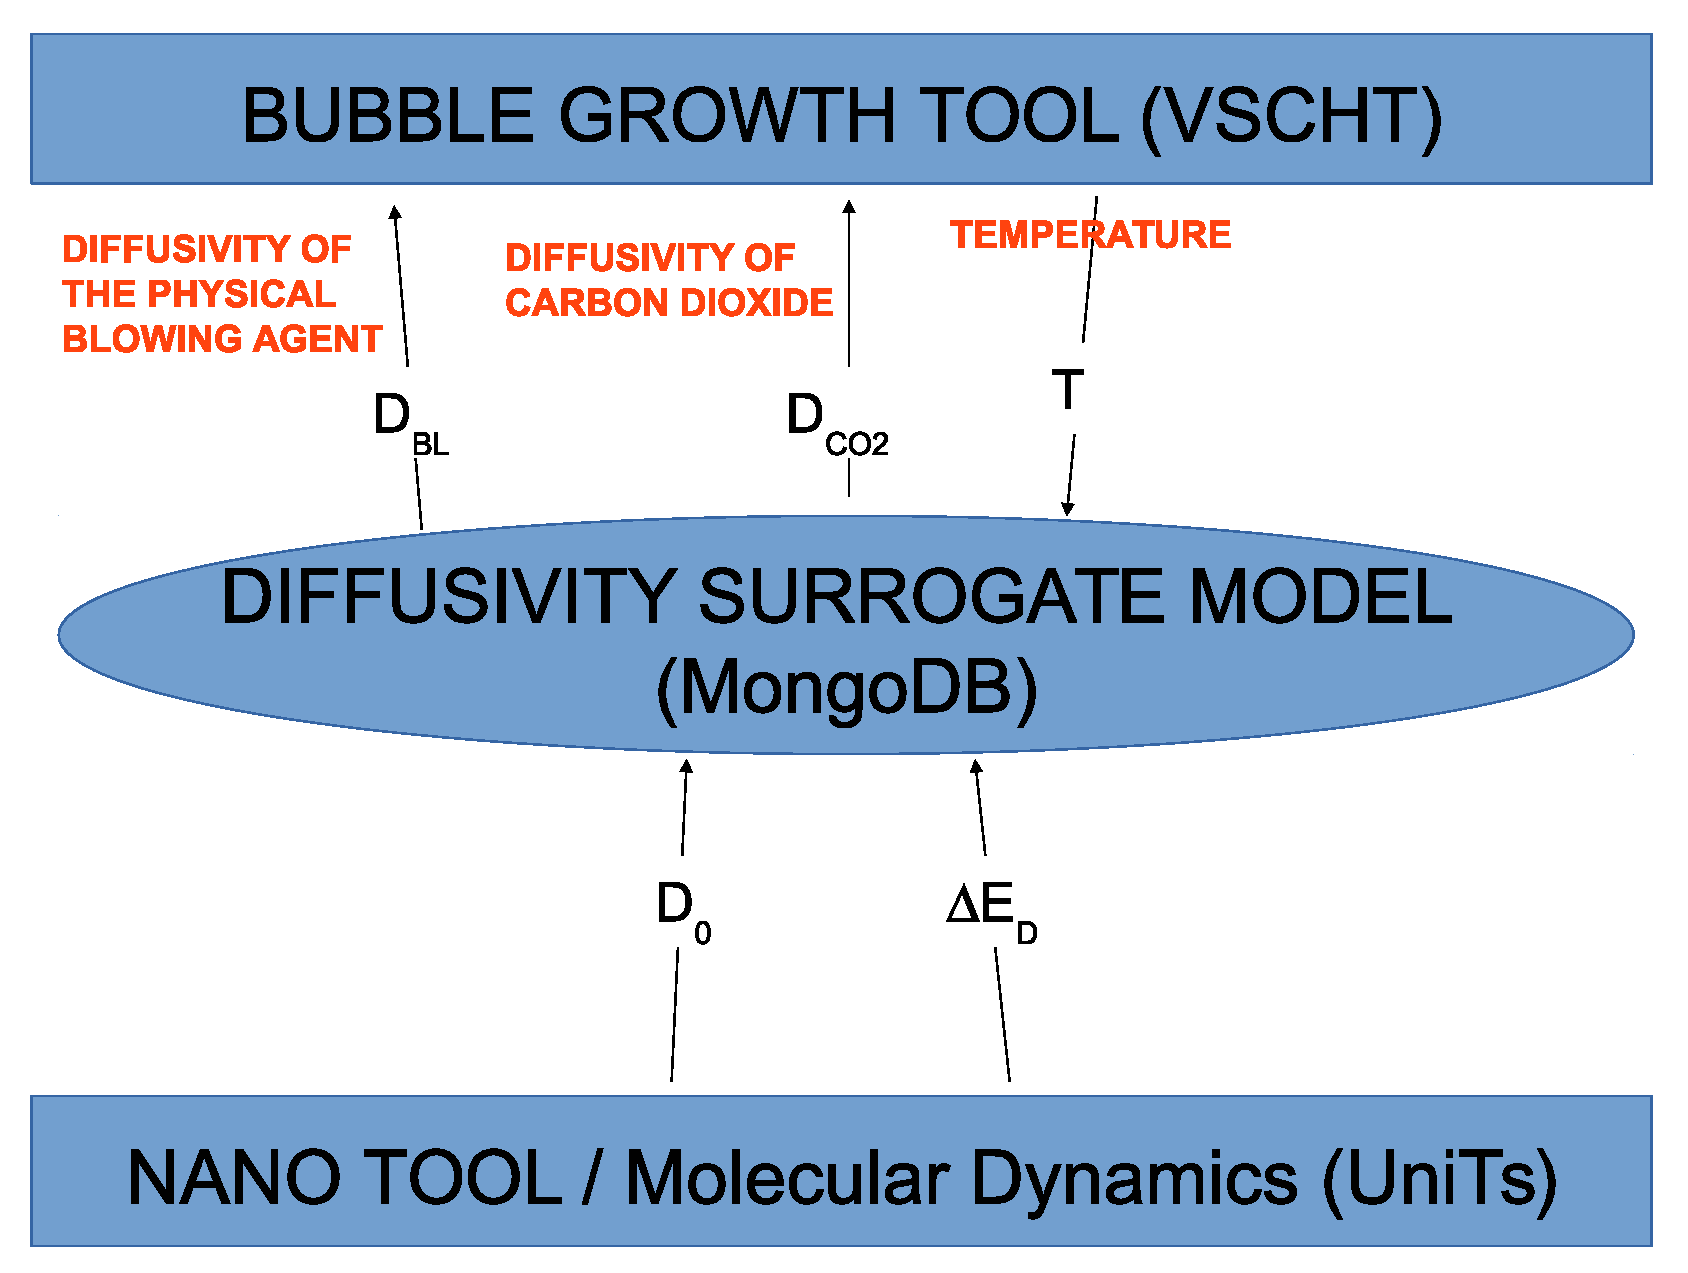
\includegraphics[width=0.48\textwidth,keepaspectratio=true]{./Content/Figures/PU_exercise_2.eps} &
    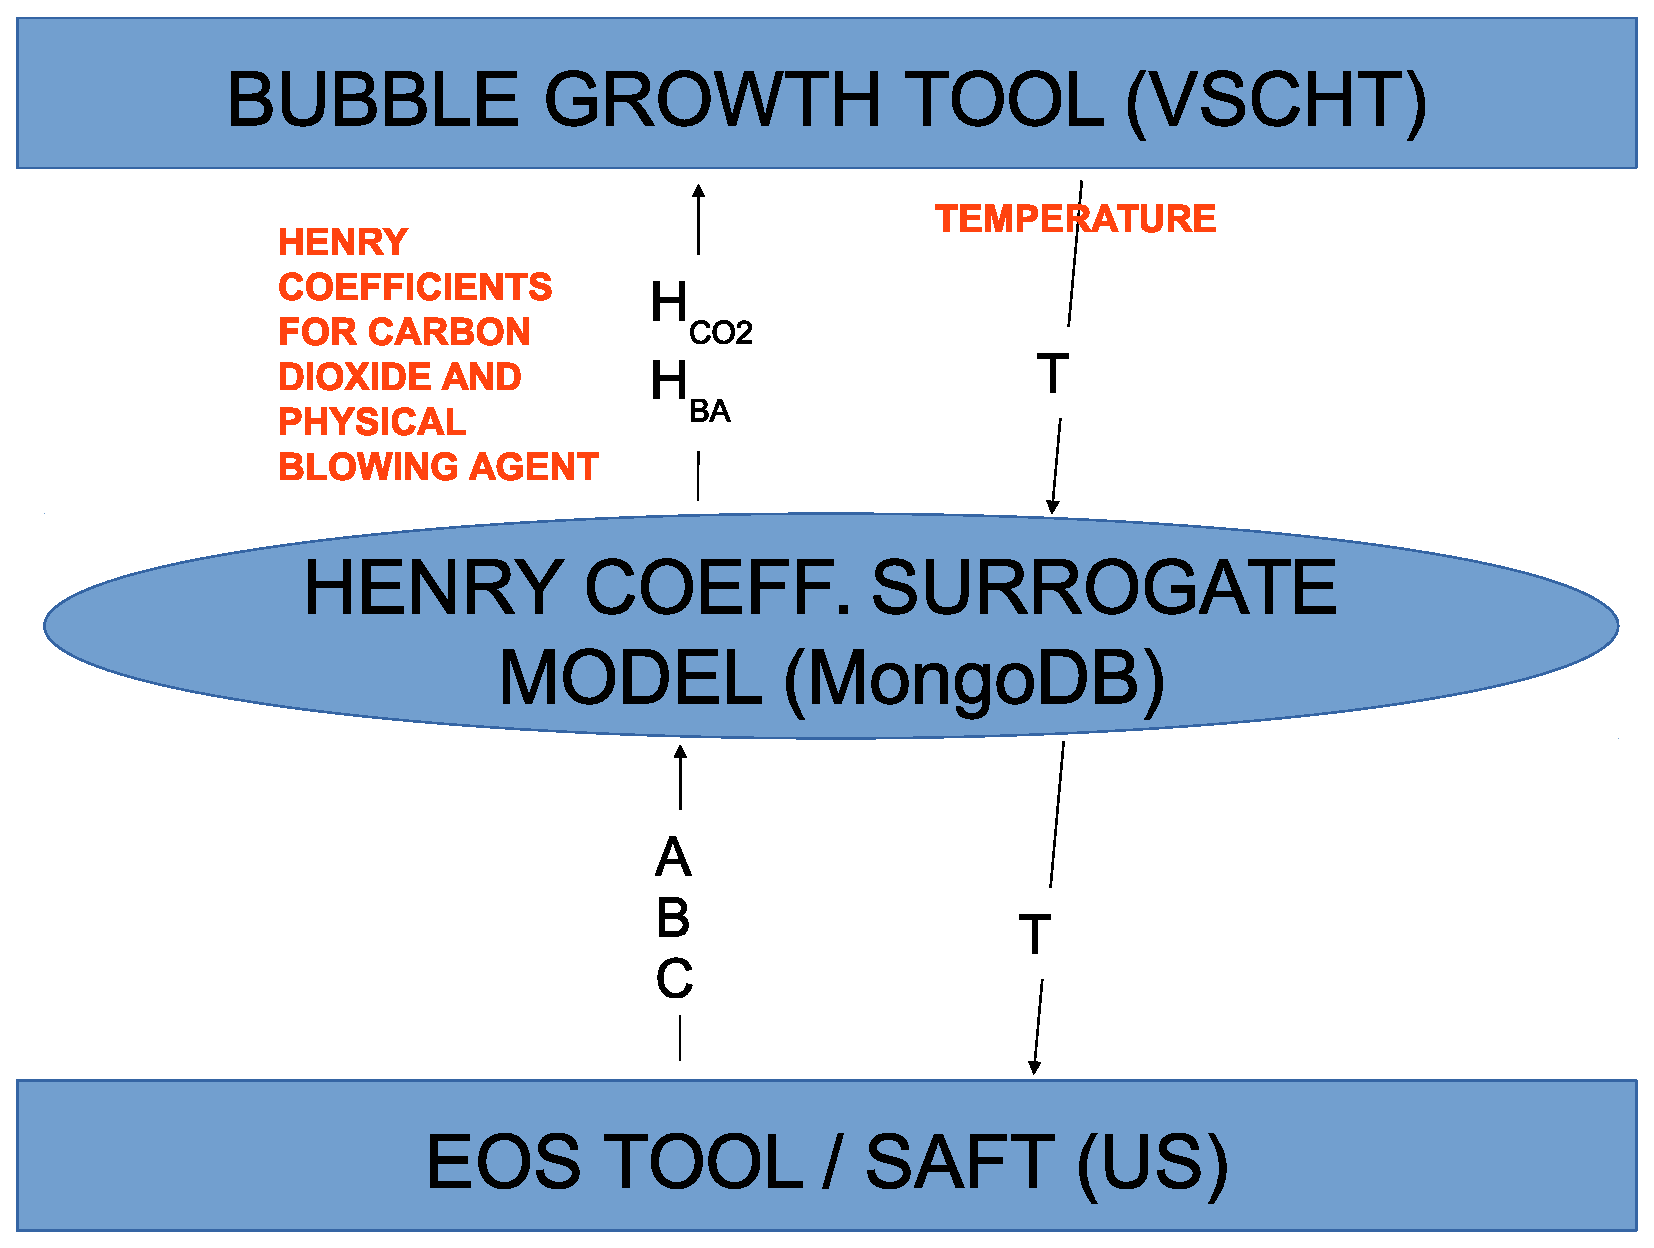
\includegraphics[width=0.48\textwidth,keepaspectratio=true]{./Content/Figures/PU_exercise_3.eps} \\

    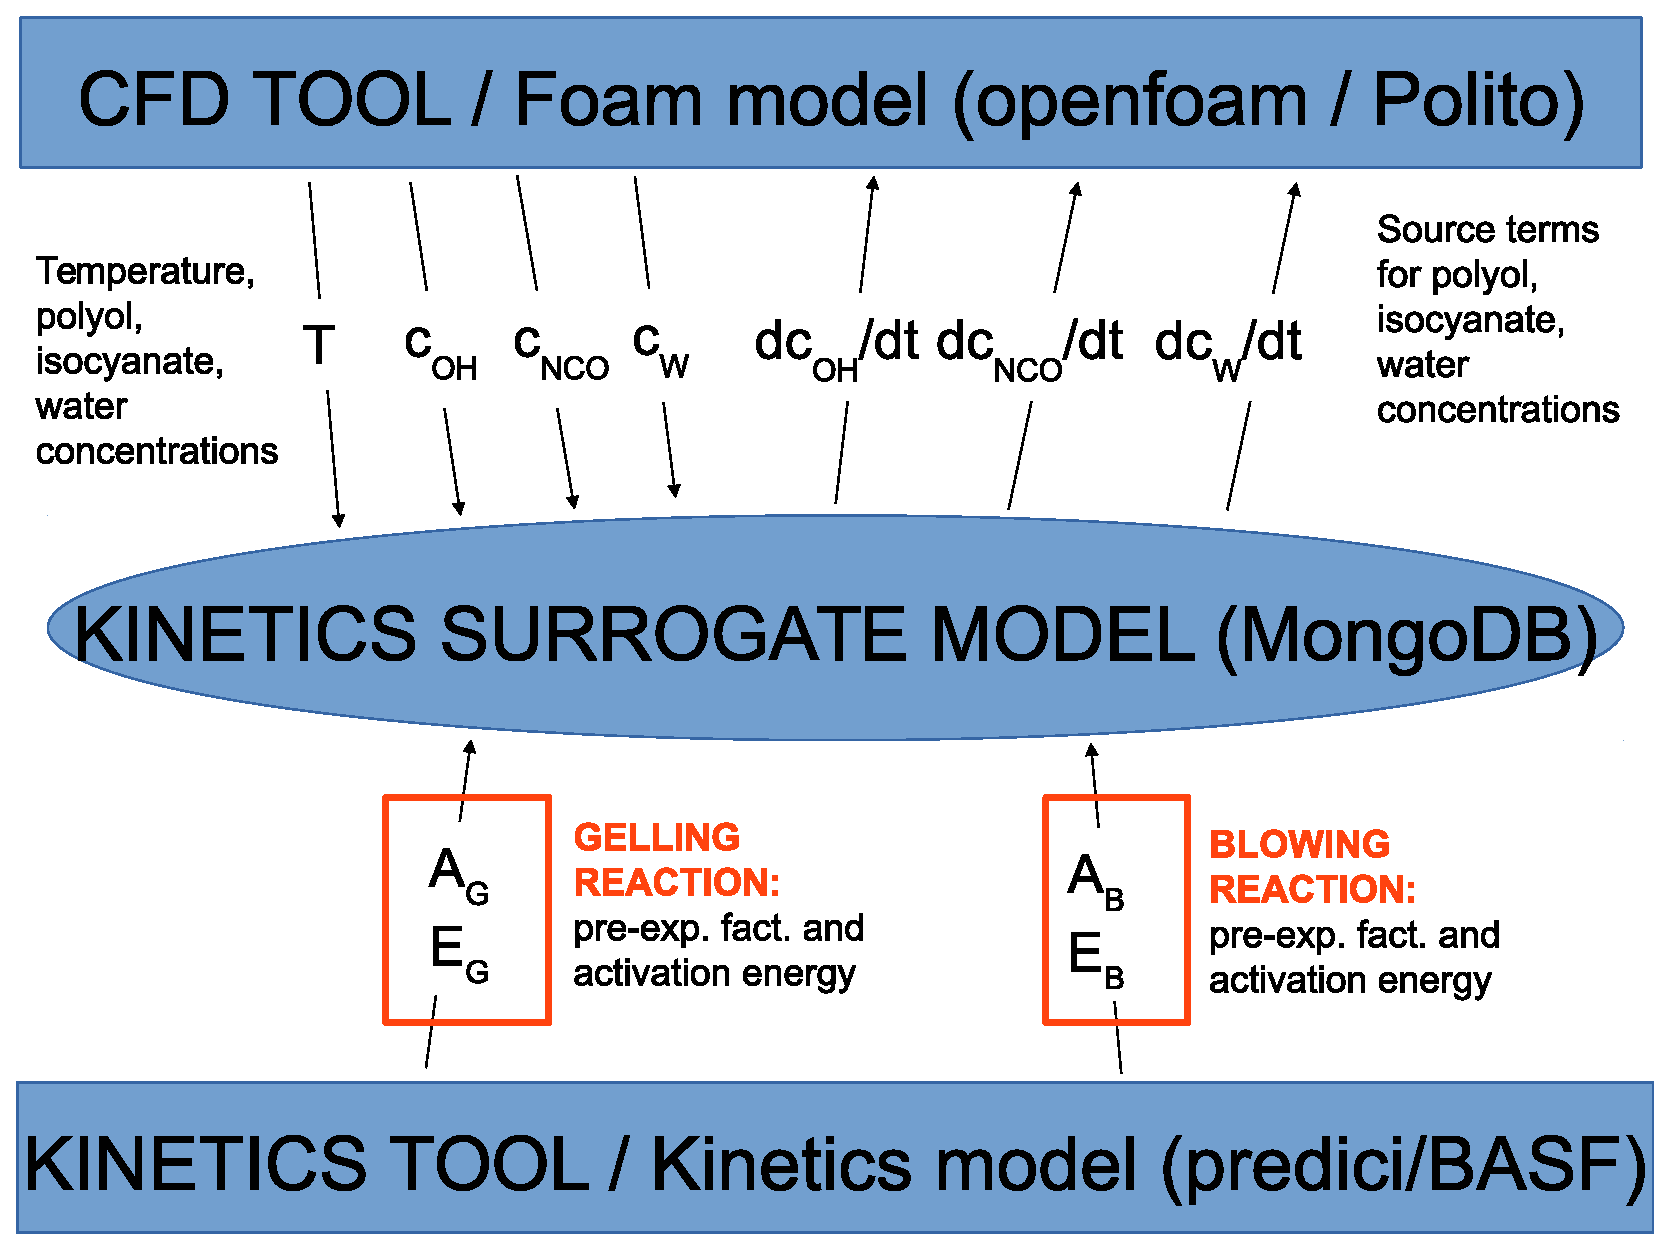
\includegraphics[width=0.5\textwidth,keepaspectratio=true]{./Content/Figures/PU_exercise_4.eps} &
    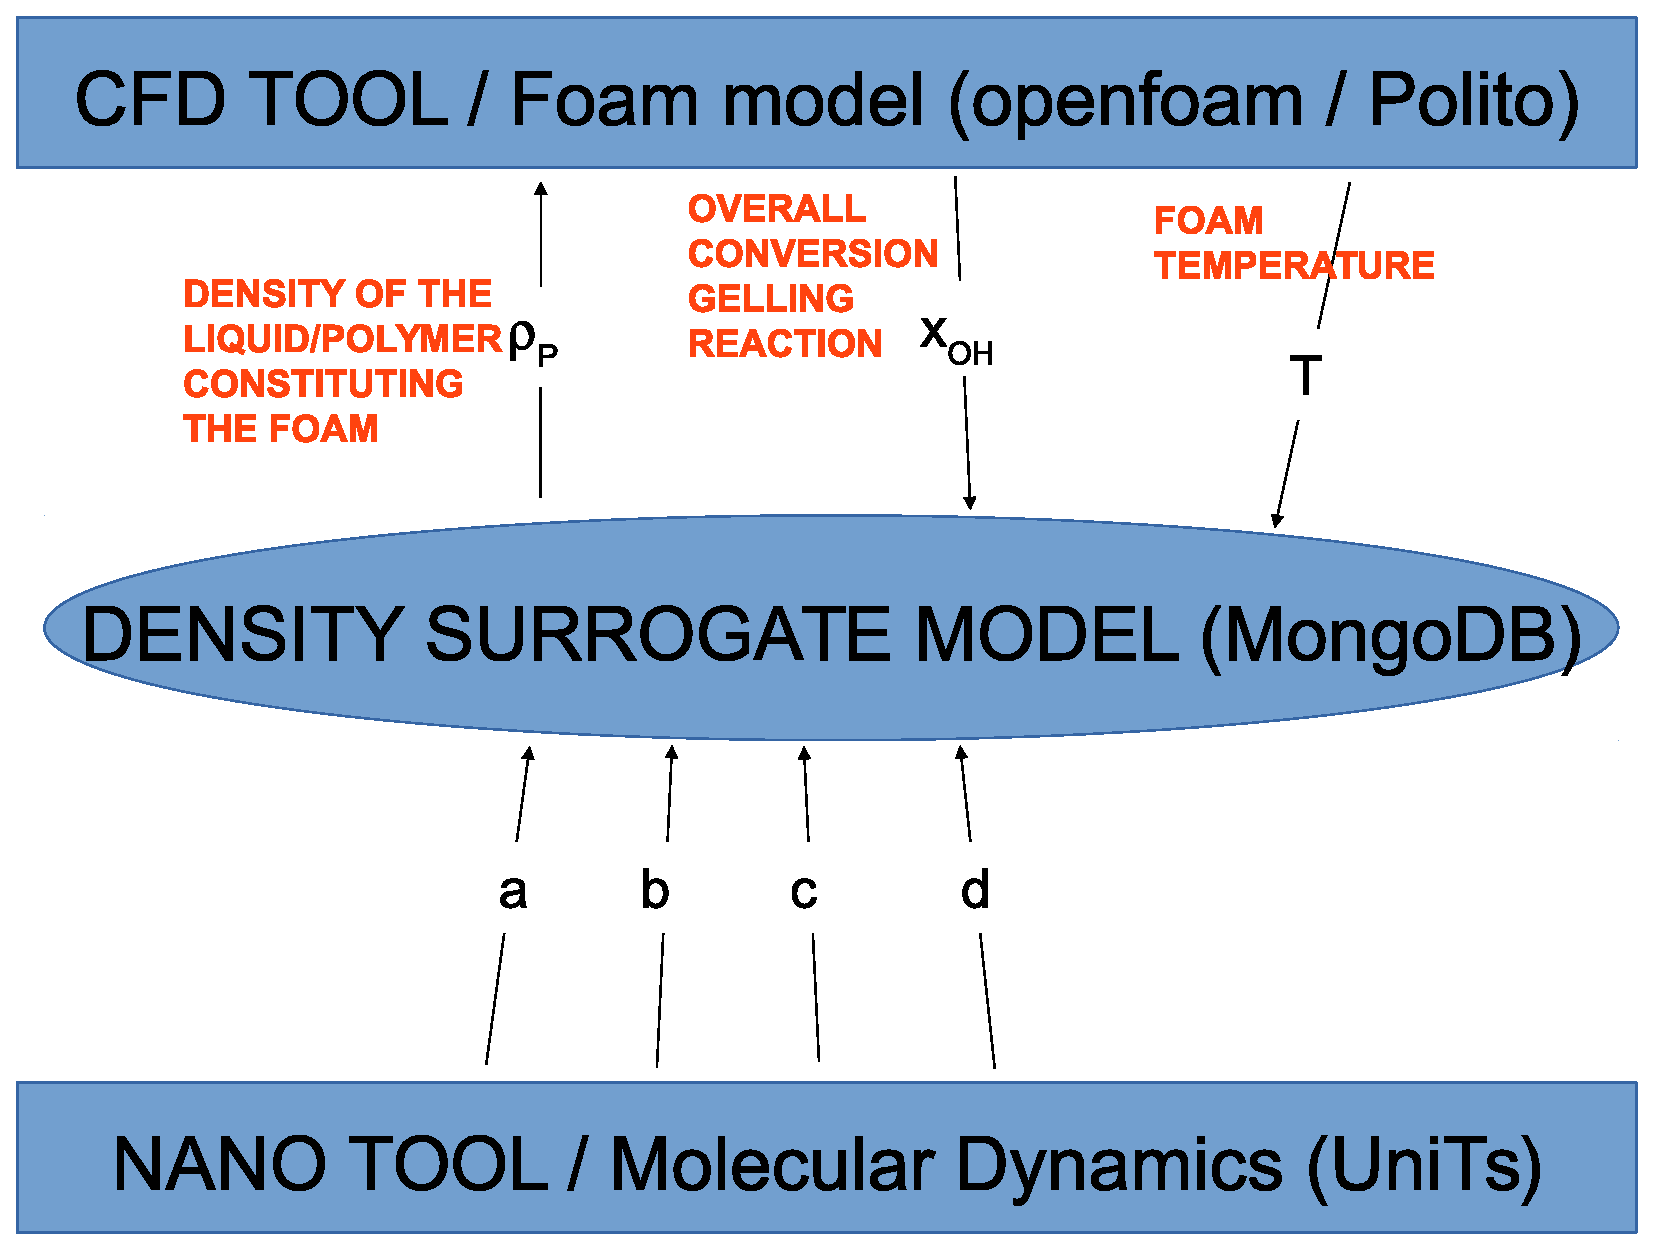
\includegraphics[width=0.5\textwidth,keepaspectratio=true]{./Content/Figures/PU_exercise_5.eps} \\

    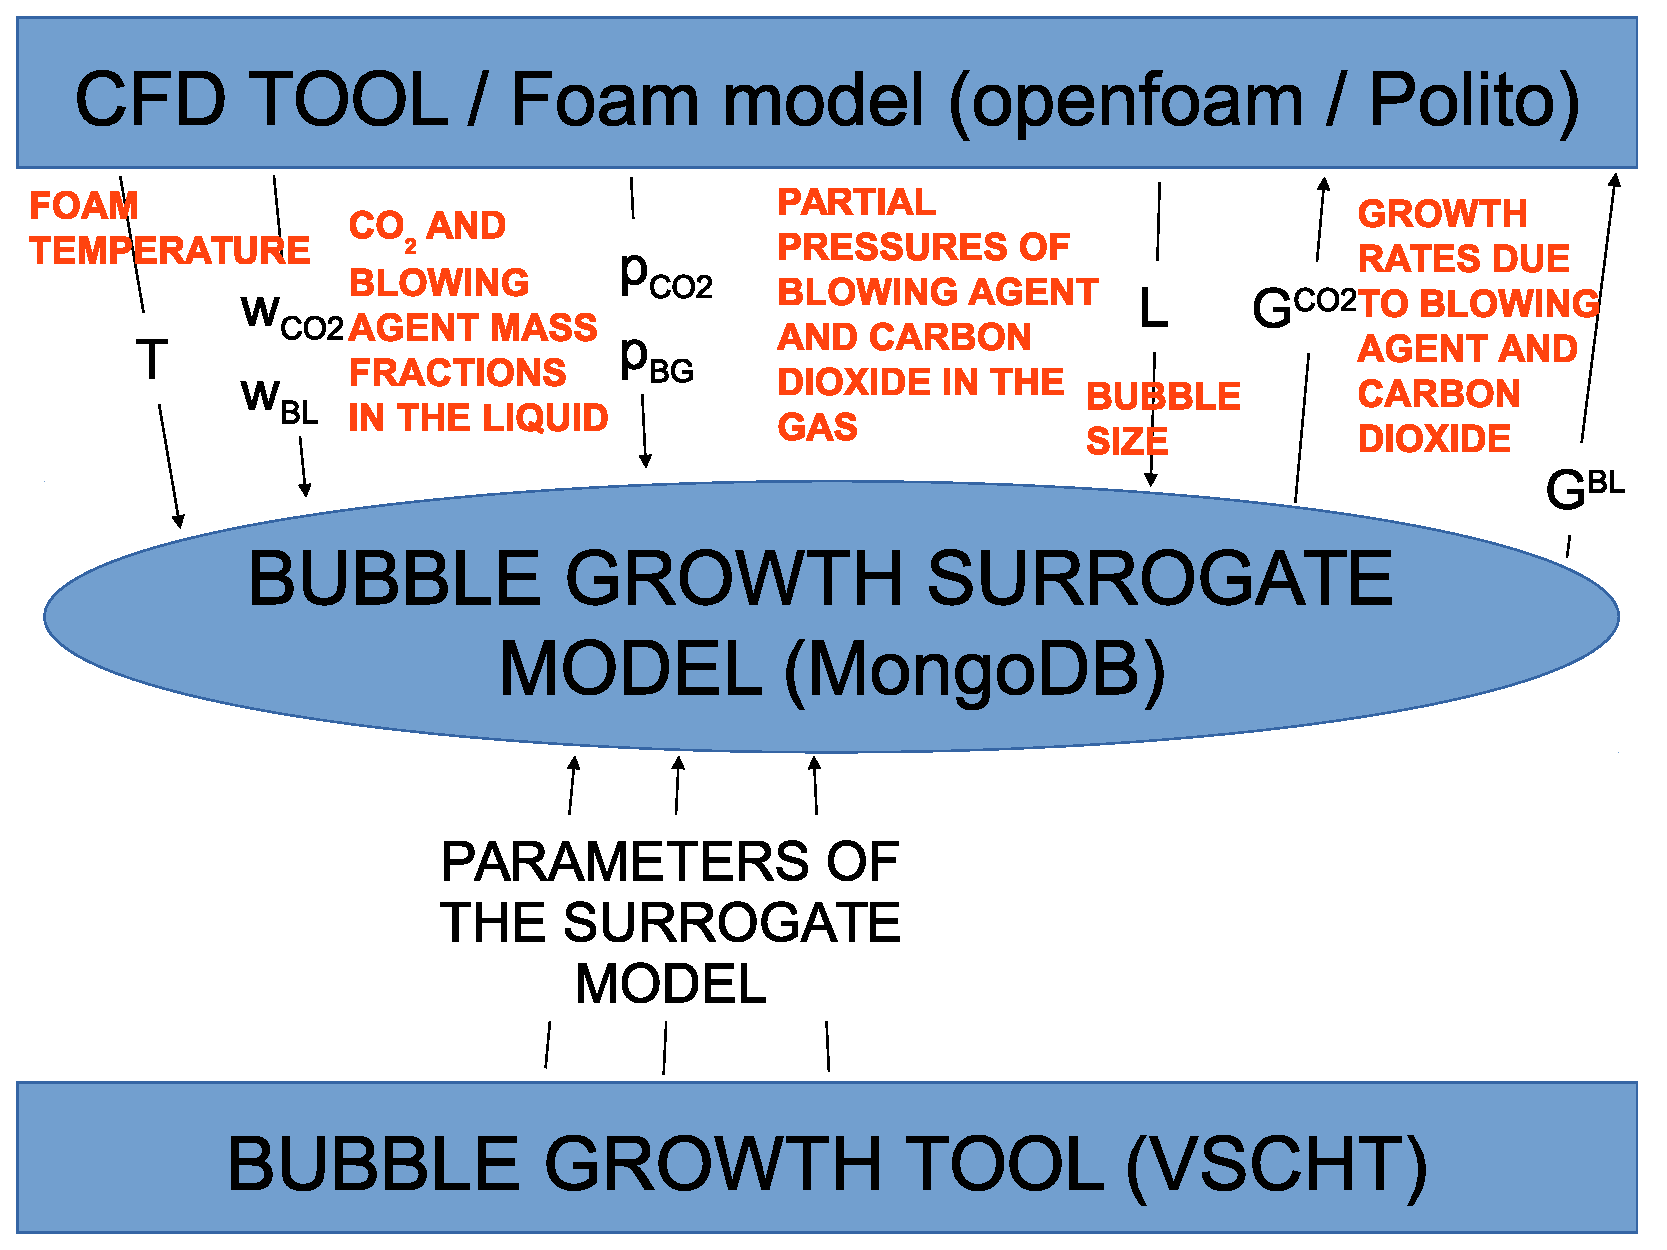
\includegraphics[width=0.5\textwidth,keepaspectratio=true]{./Content/Figures/PU_exercise_6.eps} &
    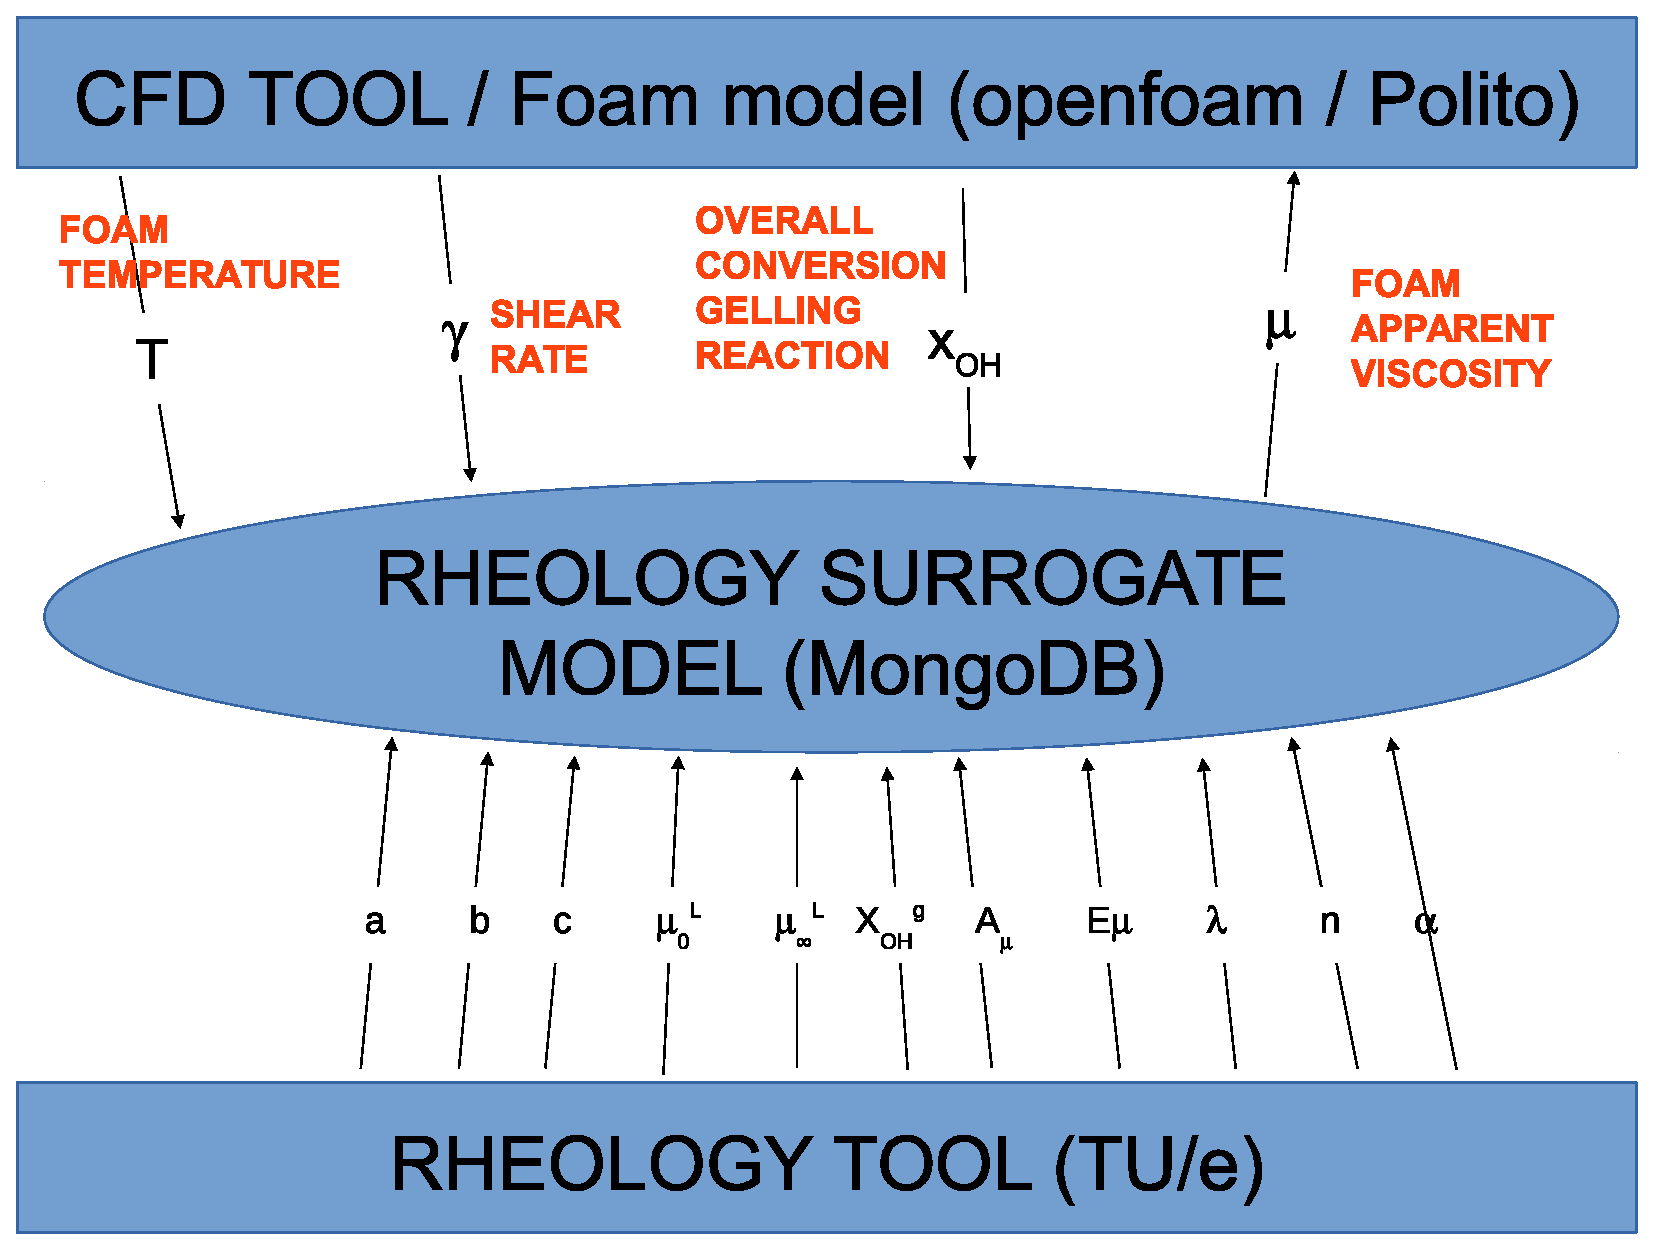
\includegraphics[width=0.5\textwidth,keepaspectratio=true]{./Content/Figures/PU_exercise_7.eps} \\
  \end{tabular}
  \caption{Layouts of links for diffusivity, Henry coefficient, kinetics, liquid
    density, bubble growth and rheology. Boxes and ellipses stand for tools and
    surrogate models, respectively.}
  \label{fig:links}
\end{figure}

The status of the recipes and adaptors (links) is summarised in Figure
\ref{fig:recipesAdaptorsStatus}.  There are 6 tools (computational fluid
dynamics, bubble growth tool, kinetics, equation of statem nano and rheology)
that are to be orchestrated in this application. 5 of the 6 tools and 3 of the 6
links are operational and have undergone testing. It is envisaged that the
remaining ones will be operational for the mid-term.

The majority tools and links scheduled for implementation in the first
application development phase are operational and have undergone testing. The
final model predictions will validated against experiments in WP6.

\begin{figure}
  \centering
  \begin{tabular}{cc}
    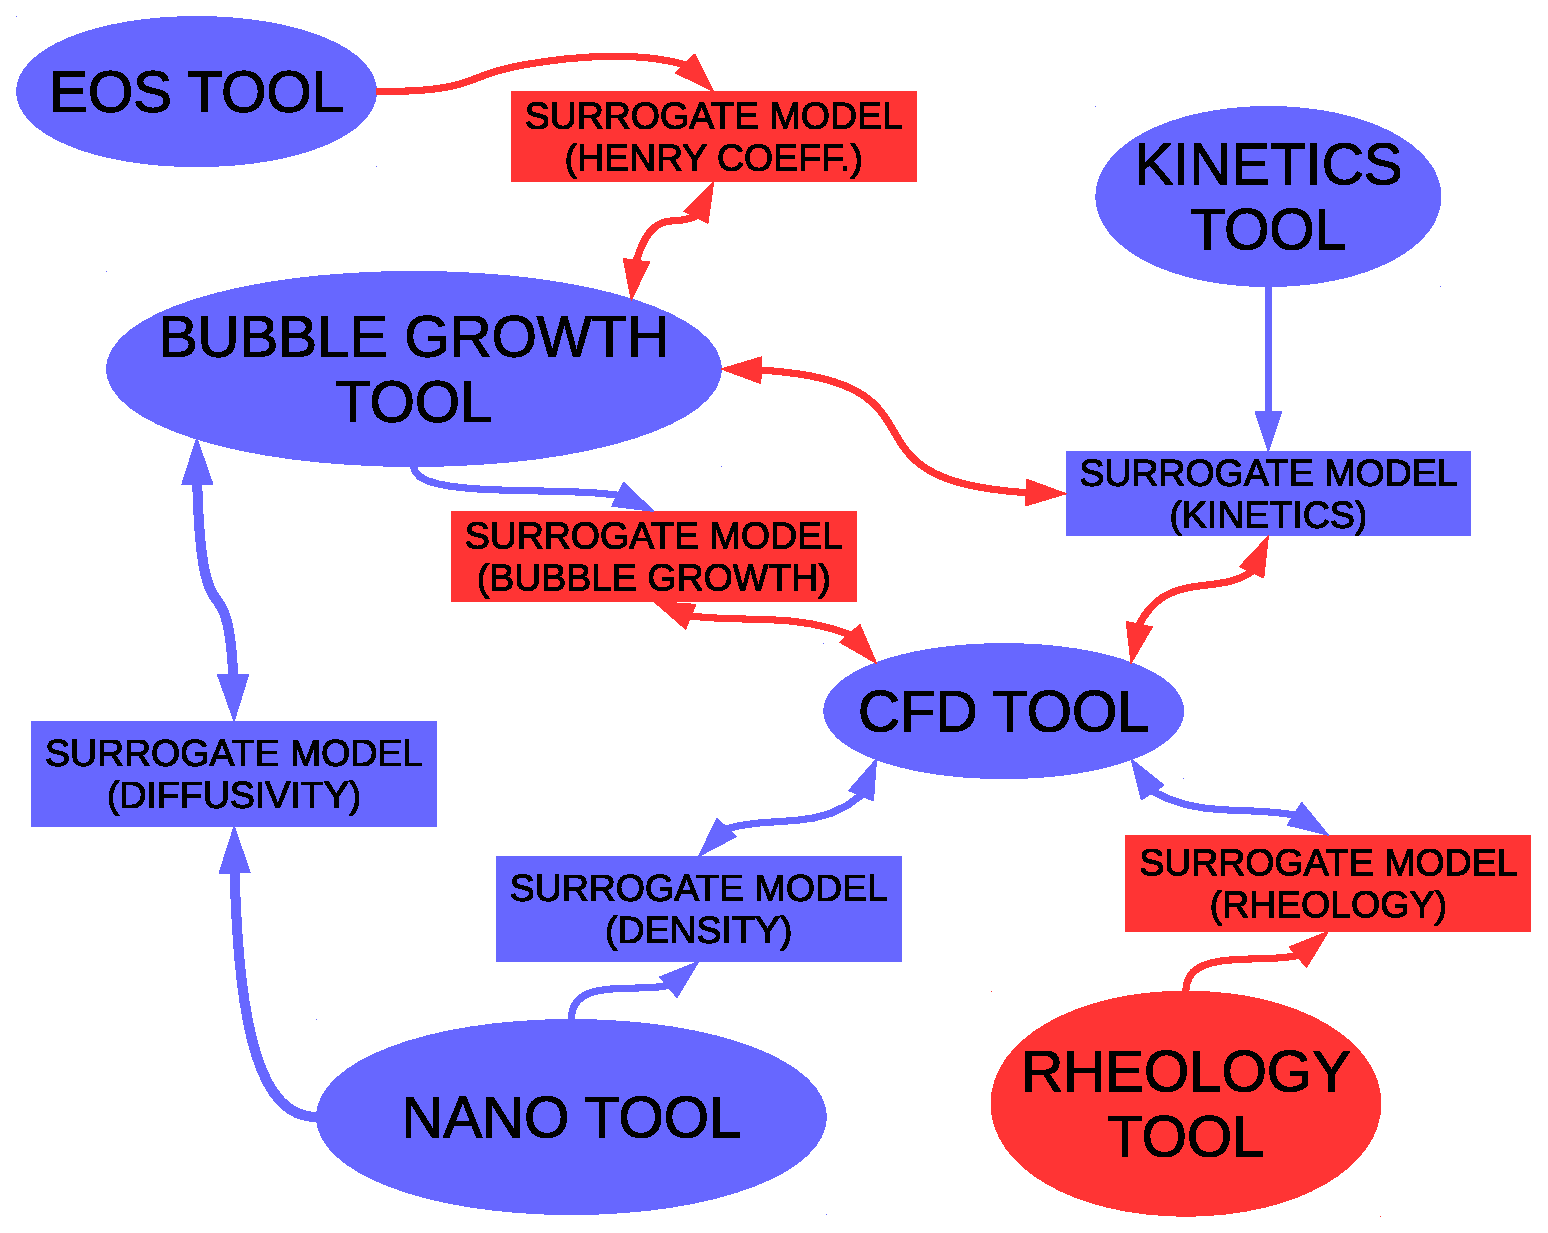
\includegraphics[width=0.70\textwidth,keepaspectratio=true]{./Content/Figures/PU_exercise_1.eps} &
    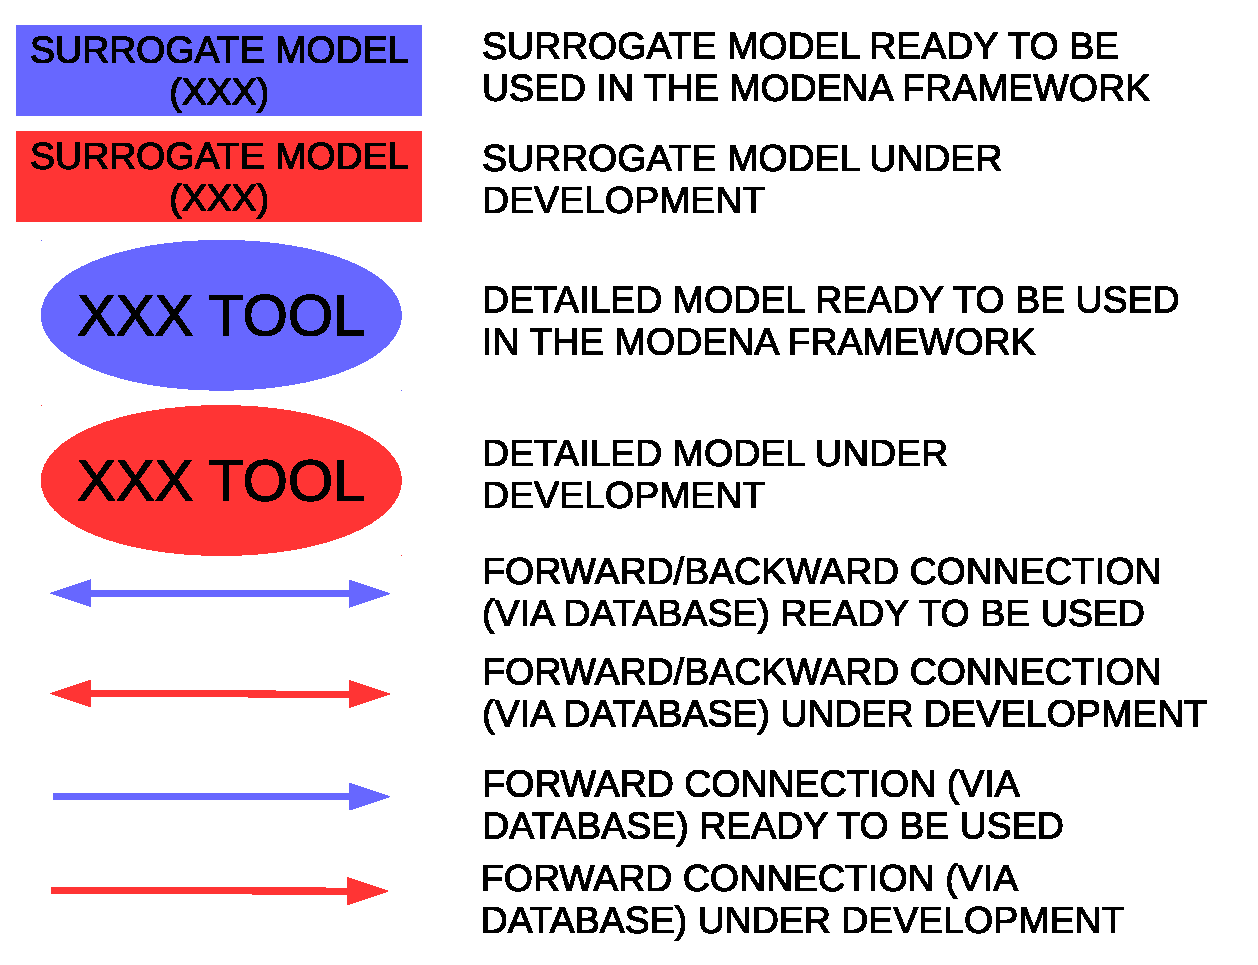
\includegraphics[width=0.27\textwidth,keepaspectratio=true]{./Content/Figures/PU_exercise_8.eps}
  \end{tabular}
  \caption{Status of recipes and adaptors.}
  \label{fig:recipesAdaptorsStatus}
\end{figure}
